\documentclass[informe.tex]{subfiles}
\begin{document}

\section{Análisis Experimental (Alonso y Gabriela)}
Diseñe y realice un análisis experimental calculando los tiempos de
ejecución en nanosegundos de sus dos soluciones para un conjunto de n puntos cuyas coordenadas
enteras están elegidas al azar en un cuadrado de 100 × 100, variando la cantidad $n$ de puntos entre
las potencias de dos de $2^3 = 8$ a $2^9 = 512$.

\subsection{Diseño}

Se diseño un script en bash \code{benchmark.sh} que realiza lo siguiente:
\begin{enumerate}
	\item \textbf{Preparación de entorno:} se ejecuta el comando \code{make}, que utiliza
	      un archivo \code{Makefile} previamente configurado para compilar todo el código implicado en
	      el proyecto.
	\item \textbf{Ejecución:} se ejecutan pruebas con n = 8, 16, 32, ..., 512
	      puntos, generados aleatoriamente con el programa \code{get\_random\_points}, en todos los
	      algoritmos implementados.
	\item \textbf{Parsing:} se utiliza el comando linux \code{sed}, de manera que se
	      encuentra el tiempo de ejecución en el output de los programas ejecutados y se guardan en un
	      archivo csv.
	\item \textbf{Análisis y Visualización:} se arma el gráfico con ayuda de código en python que
	      recibe el archivo csv y muestra los resultados para su análisis.
\end{enumerate}

\subsection{Realización}

Gráfico de ejemplo de resultados esperados:
\begin{figure}[h]
	\centering 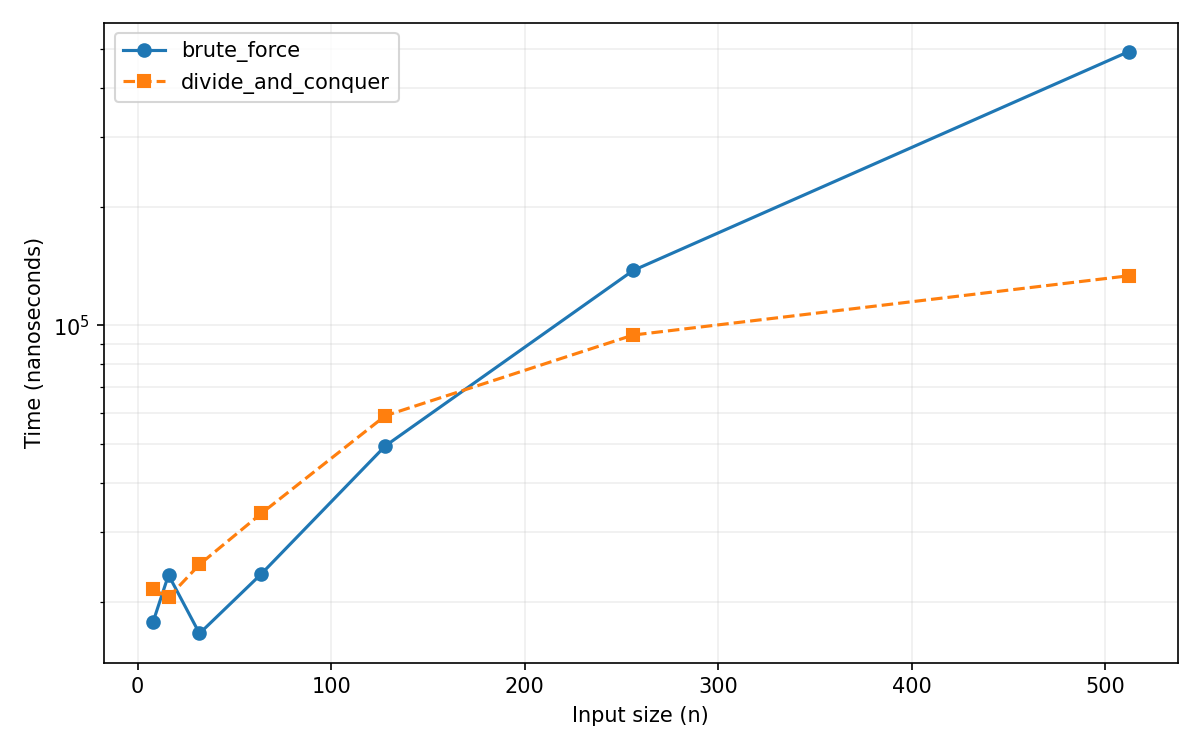
\includegraphics[width=0.8\textwidth]{img/plot_bf_dv.png}
\end{figure}
Como podemos comprobar a simple vista, efectivamente \code{divide\_and\_conquer} presenta un menor
complejidad temporal que se pronuncia con una mayor cantidad de puntos.

\end{document}
